\documentclass[a4paper, 12pt]{article}

%\usepackage{savetrees}
\usepackage{graphicx}
\graphicspath{{./images/}}
\title {Student Robotics 2009\\ Slug Documentation}
\date{\today}
\setcounter{tocdepth}{1}


\begin {document}

\maketitle

\noindent This document describes the functions of the Slug

\section{Board Outline}

Figure \ref{slug-outline} illustrates the outline of the slug casing on a 1:1 scale.

\begin{figure}[ht]
\begin{center}
\includegraphics[keepaspectratio, scale=1, trim = 7cm 10cm 5cm 12cm]{./images/slugcase.png}
\caption{\label{slug-outline}The board outline of the slug}
\end{center}
\end{figure}

\section{Brief Description}

The slug is a modified version of Linksys' NSLU2. It acts as the central processing unit for the robot. It connects directly to the power board which is where it sources its power and communicates over I2C with the board.

\clearpage
\newpage

\section {Pin out}

The following section provides the pin-out of the umbilical cord as illustrated in figure \ref{slug-pinout}.

\begin{figure}[ht]
\begin{center}
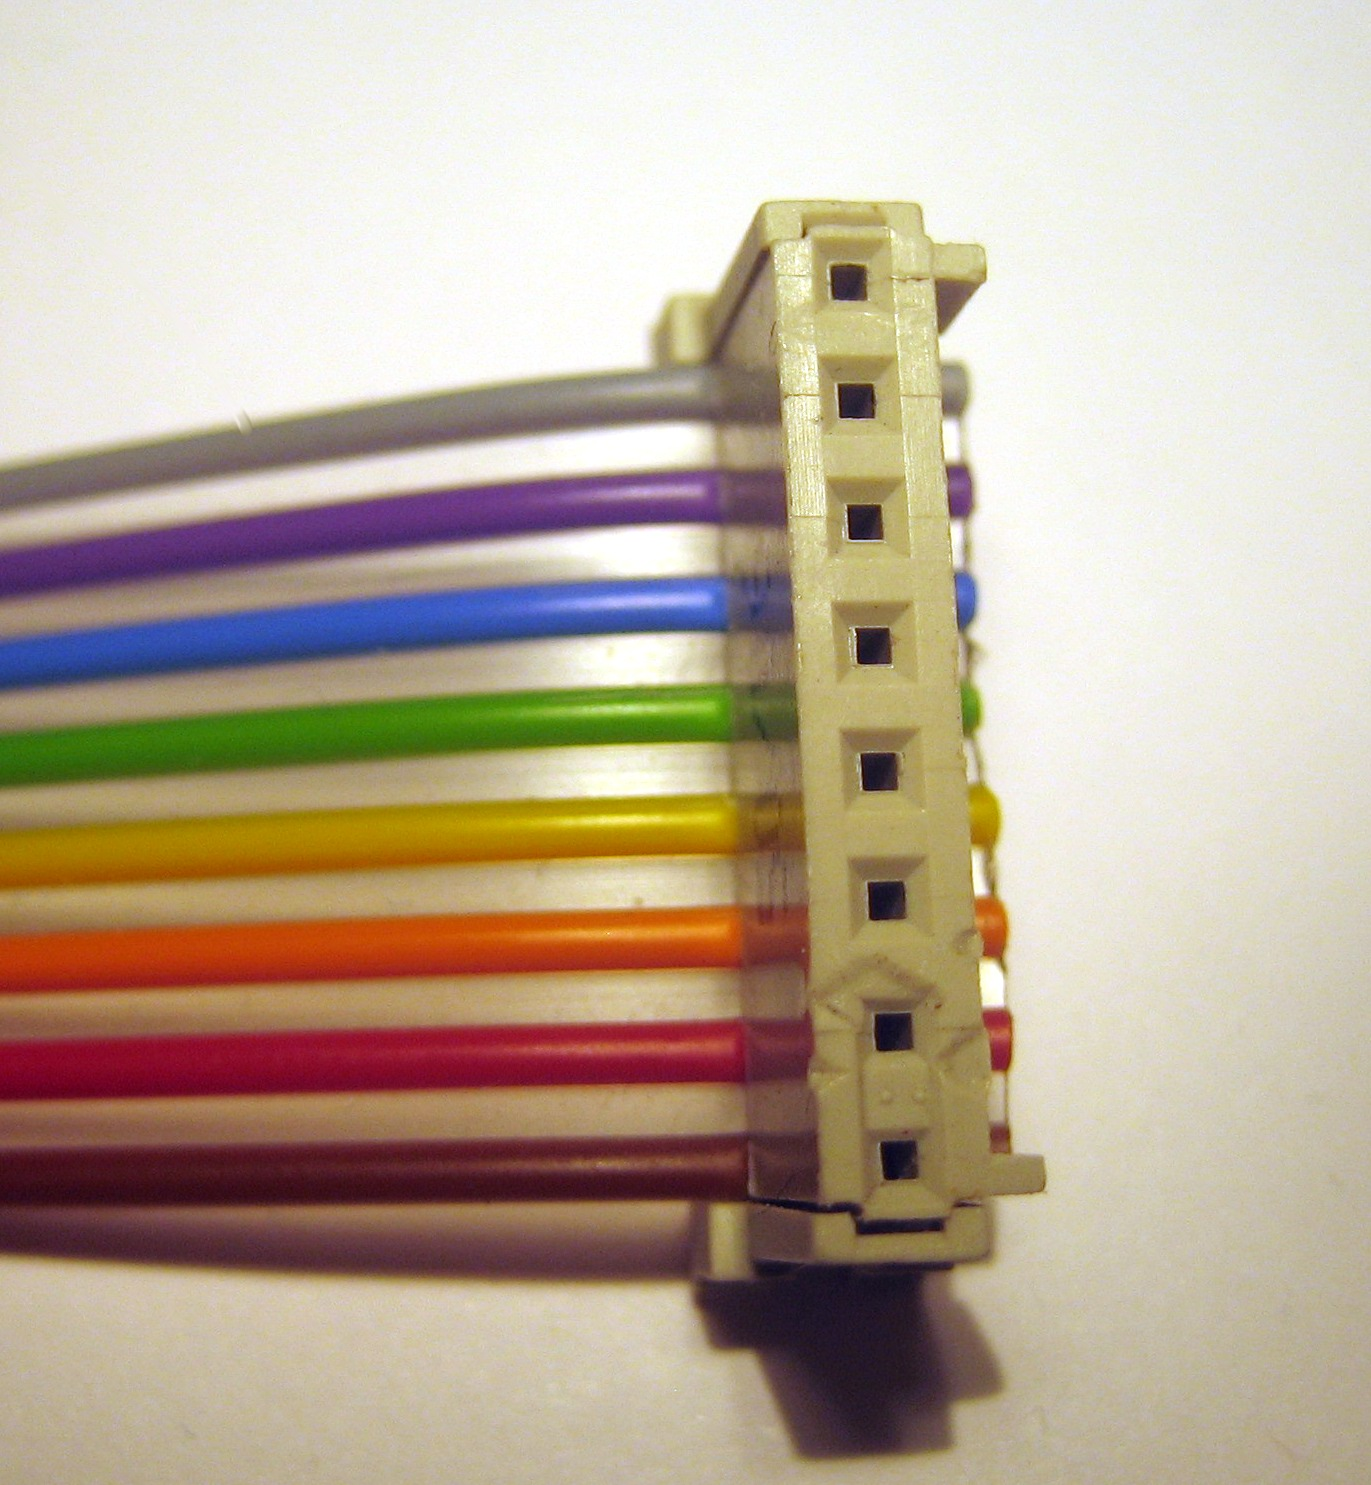
\includegraphics[keepaspectratio, width=7cm]{./images/slugpins.png}
\caption {\label{slug-pinout}Slug pin-out}
\end{center}
\end{figure}

\begin{center}
\begin{tabular}{|c|c|c|}
\hline
\textbf {Pin Number} & \textbf {Wire Colour} & \textbf {Description}\\
\hline
1 & Grey & GND\\
2 & SCL & Violet\\
3 & SDA & Blue\\
4 & Xbee to Slug & Green\\
5 & Slug to Xbee & Yellow\\
6 & Slug Boot Pin & Orange\\
7 & VREGSLUG2 & Red\\
Not Connected & Not used & Brown\\
\hline
\end{tabular}
\end{center}

\section {Boot}

THe slug boots in X seconds using firmware version X.

\end {document}
